\section{Considerações iniciais}

Neste capítulo são destacados os tópicos mais relevantes para a compreensão da metodologia e análise dos resultados desse trabalho, com foco na preparação das imagens para a extração de características. O problema do desbalanceamento de classes e seu efeito na classificação também são abordados, assim como a extração de características para compreender as propriedades extraídas das imagens. Alguns trabalhos relacionados são utilizados como exemplo, com o objetivo de elucidar tais tópicos.

Inicialmente, a Seção~\ref{sec:preprocessamento} apresenta alguns dos principais métodos utilizados para o pré-processamento de imagens (i.e.\ remoção de ruído, realce de imagens e convolução), relevantes para o desenvolvimento desta pesquisa. Após, a extração de características é definida na Seção~\ref{sec:extracao}. Tendo como proposta melhor compreender o problema do desbalanceamento de classes, a Seção~\ref{cap:desbalanceamento} exemplifica as operações utilizadas para o rebalanceamento. Nessa seção, além de caracterizar o problema, são apresentadas duas vertentes para solucioná-lo: sobreamostragem e subamostragem. A seção seguinte (\ref{sec:classificacao}) apresenta o classificador de padrões utilizado e a Seção~\ref{sec:reducaodimensionalidade} aborda dois métodos de redução de dimensionalidade utilizados nos experimentos.

%--------------------------------------------------------------------------------
\section{Pré-processamento de imagens}
\label{sec:preprocessamento}

Uma imagem digital $I$ pode ser definida como uma função $f(x,y)$, onde $x$ e $y$ são as coordenadas cartesianas de um determinado ponto e $f$ a intensidade (brilho) da imagem naquele ponto. Essa imagem é composta por finitos elementos chamados de pixels que podem ser diretamente acessados através de sua posição $x$ e $y$. Digitalmente, uma imagem é representada por uma matriz de valores com $M$ linhas e $N$ colunas onde cada elemento representa a sua intensidade. Uma imagem colorida $I$ do sistema RGB possui três canais de cores representantes das cores vermelha, verde e azul. Cada elemento $I(x,y)$ corresponde a uma tripla $(r, g, b)$ de números, com $0 \leq r \leq 255$, $0 \leq g \leq 255$ e $0 \leq b \leq 255$, onde 0 é a intensidade de cor mais escura e 255 a mais clara. A combinação dessas intensidades resulta na cor do pixel \cite{Gonzalez2007}. A Figura \ref{fig:pixel} mostra uma visualização ampliada dos pixels de uma imagem digital.

\begin{figure}[!htbp]
 \begin{center}
   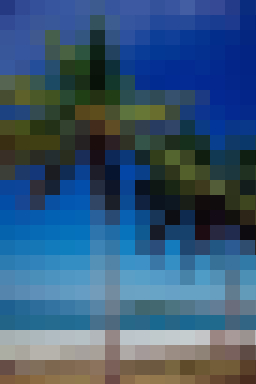
\includegraphics[width=0.4\linewidth]{figuras/pixel.jpg}
 \caption[Visualização pixelizada de uma imagem da base COREL-1000.]{Visualização pixelizada de uma imagem da base COREL-1000\footnotemark. \\ \textit{Fonte:~Elaborado pela autora.}}
 \label{fig:pixel}
 \end{center}
\end{figure}
\footnotetext{Disponível em \url{http://wang.ist.psu.edu/docs/related/}}

O processo de aquisição por um sistema de imageamento pode causar diversas imperfeições nas imagens, como pixels ruidosos, brilho inadequado e outras degradações. O pré-processamento de imagens é caracterizado por receber uma imagem de entrada e fornecer uma imagem de saída. Nessa etapa, efeitos indesejáveis podem ser eliminados e certas características realçadas (Figura \ref{fig:preproc}). Considera-se que um determinado critério utilizado para uma imagem pode não ser o mais eficiente para outra, dependendo assim da área de aplicação.

\vspace{12pt}
\begin{figure}[!htbp]
 \begin{center}
   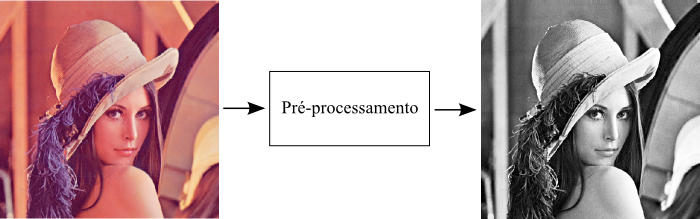
\includegraphics[width=1\linewidth]{figuras/preprocessamento.png}
 \caption[Sobre a imagem RGB de entrada foram realizadas operações de borramento, realce e de equalização de histograma. A imagem à direita é resultante dessas operações.]{O pré-processamento de imagens é caracterizado por receber uma imagem como entrada e fornecer uma imagem de saída. Sobre a imagem RGB de entrada (à esquerda) foram realizadas operações de borramento, realce e de equalização de histograma. A imagem à direita é resultante dessas operações. \textit{Fonte:~Elaborado pela autora.}}
 \label{fig:preproc}
 \end{center}
\end{figure}

Assim, técnicas de pré-processamento tornam os dados mais adequados para posterior análise, ao eliminar ou reduzir problemas como ruídos e imperfeições. Em \citeonline{Ponti2010}, o autor relata que a utilização de métodos de restauração na etapa de pré-processamento da imagem, antes da segmentação, resultou em uma qualidade superior para todos os testes, com valores de erro e desvio padrão menores. No referido estudo, métodos de realce causaram perda de informação e por isso não são indicados para uso em imagens obtidas por microscópio. O método indicado para evitar a amplificação de ruído nessas imagens é o algoritmo iterativo Richardson-Lucy ~\cite{Ponti-Jr2011}. Esse método de restauração utiliza um processo iterativo para recuperar uma imagem degradada que foi borrada por algum processo conhecido. Utiliza uma metodologia probabilística, baseada em \sigla{EM-ML}{\textit{Expectation-Maximization Maximum Likelihood}}, para encontrar uma imagem que maximize a probabilidade de se visualizar a imagem original sem degradação, considerando um modelo de ruído de Poisson. Algoritmos iterativos como o Richardson-Lucy tem a vantagem de permitir soluções parciais, evitando amplificação de ruído.

Em contrapartida, \citeonline{6} propuseram uma representação para imagens faciais baseada em características de textura, sem utilizar pré-processamento. Este aparece somente como sugestão de trabalho futuro, como possível correção de problemas do sistema de captura (i.e. suavização causada pela captura fora de foco). O que implica que, apesar dos bons resultados, a melhoria com a utilização de pré-processamento não foi investigada. Pode-se imaginar, portanto, que o uso de pré-processamento pode melhorar os resultados já obtidos, através do realce de textura e eliminação de imperfeições nas imagens.

Como exemplo do uso de métodos de pré-processamento, considere imagens de algas verdes obtidas por um microscópio de alta resolução. Essas algas são mergulhadas em um líquido que normalmente causa problemas de ruído e pouco contraste. Para a preparação dessas imagens, antes da extração de características, \citeonline{Borges2013} cita algumas etapas comuns em processamento de imagens digitais:

\begin{enumerate}
\item As imagens -- originalmente em RGB -- são convertidas para uma escala de cinza;
\item A dimensão da imagem é reduzida para diminuir o tempo de execução dos passos subsequentes de processamento;
\item O constraste é ``ajustado'', para aumentar a diferença das intensidades dos pixels da imagem e corrigir o brilho;
\item A imagem é filtrada, removendo ruídos causados pelo processo de captura;
\item O contorno é realçado, pois a forma é uma das características mais importantes para discriminar algas (e outros objetos);
\item Por fim, o histograma é equalizado.
\end{enumerate}

\citeonline{Xu2016} propuseram um método de pré-processamento de imagens de faces com o objetivo de gerar imagens sintéticas para posterior reconhecimento de padrões. Inicialmente, o método separa uma imagem em metade-esquerda e metade-direita e espelham a metade-direita. Após, um algoritmo de gradiente descendente iterativo é utilizado para atualizar os vetores que representam cada metade, otimizando-os. Por fim, esses vetores são concatenados para compor uma nova face do mesmo tamanho da imagem original. Os resultados são apresentados como estado da arte para o pré-processamento de imagens de face para a tarefa de reconhecimento.

Esses estudos evidenciam a importância da etapa de pré-processamento de imagens, indicando que o tratamento das imagens antes da extração de características pode melhorar os resultados obtidos.

%--------------------------------------------------------------------------------
\subsection{Filtragem espacial e convolução}

% %--------------------------------------------------------------------------------
% \subsection{Convolução}
\label{sec:convolucao}

Um filtro espacial, também conhecido como \textit{kernel}, máscara ou janela, consiste em uma matriz de vizinhanças e uma operação a ser realizada nos pixels de uma imagem. A filtragem cria um novo pixel com as mesmas coordenadas do centro da vizinhança, contendo o valor resultante da filtragem. Dessa forma, a imagem filtrada contém os pixels resultantes da passagem do centro do filtro espacial por todos os pixels da imagem original. O processo de percorrer a imagem com um filtro espacial é chamado de correlação. A convolução, que pode ser definida como o operador $*$ em

\begin{equation*}
\text{mapa de características} = \text{imagem de entrada} * \text{filtro},
\label{eq:conv}
\end{equation*}

\noindent trata-se do mesmo processo, mas com o filtro previamente rotacionado em $180^{\circ}$ \cite{Gonzalez2007}.

Os métodos de filtragem possuem como objetivo aperfeiçoar certos aspectos da imagem de entrada. Essa filtragem pode ser realizada no domínio da frequência ou no domínio espacial. Um filtro de suavização típico no domínio espacial é o de Gaussiana, que resulta no borramento e redução de ruído, a fim de remover detalhes da imagem (Figura~\ref{fig:blur}). Esse filtro utiliza uma função Gaussiana para calcular a transformação a ser realizada em cada pixel. A equação que representa a função Gaussiana em duas dimensões é definida por
\begin{equation*}
    G_{\sigma}(x,y) = \frac{1}{2\pi \sigma^2} e^{-\frac{x^2 + y^2}{2 \sigma^2}},
\label{eq:Gaussian}
\end{equation*}

\noindent onde $x,y$ são coordenadas de um determinado pixel da imagem e $\sigma$ o desvio padrão que determina o raio da distribuição Gaussiana aplicada. Valores altos de variância ($\sigma^2$) fazem com que o resultado da função se aproxime da média.

% A filtragem Gaussiana seletiva objetiva borrar áreas da imagem onde há pouco detalhe, porém preservando contraste e pequenas estruturas. Esse tipo de filtragem é dita adaptativa, pois modifica-se o parâmetro $\sigma$ (Equação~\ref{eq:Gaussian}) para cada pixel da imagem. Uma implementação dessa técnica utiliza a variância global da imagem $\sigma_g$ e variâncias locais $\sigma_r$, suavizando com maior intensidade regiões onde a $\sigma_r \leq \sigma_g$, e suavizando menos as regiões onde $\sigma_r > \sigma_g$.

\vspace{12pt}
\begin{figure}[!hbpt]
  \subfloat[Original]{ 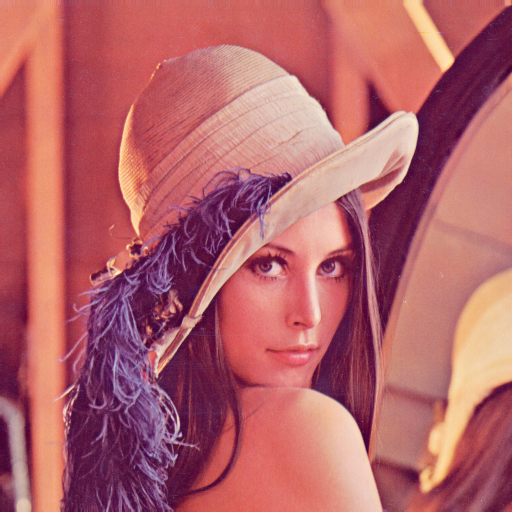
\includegraphics[width=.49\linewidth]{\detokenize{figuras/original.png}}
  }
  \subfloat[Filtrada]{
    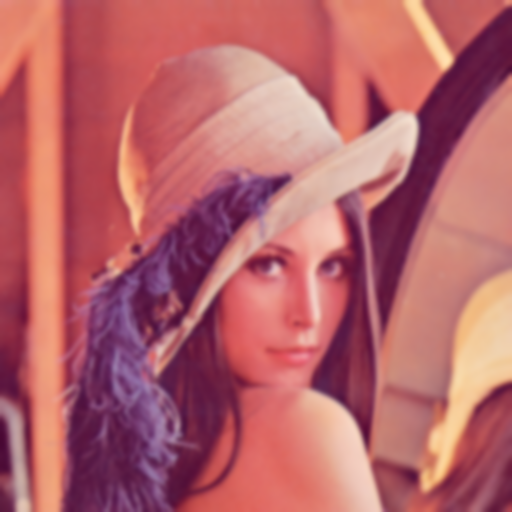
\includegraphics[width=.49\linewidth]{\detokenize{figuras/blur.png}}
  }
 \caption[Exemplo de filtragem Gaussiana como operação de pré-processamento.]{Exemplo de filtragem gaussiana como operação de pré-processamento. \textit{Fonte:~Elaborado pela autora.}}
 \label{fig:blur}
\end{figure}

%--------------------------------------------------------------------------------
% \subsection{Deconvolução}
% \label{sub:deconvolucao}
%
% O processo de convolução, descrito na seção anterior, também pode ser definido como a passagem de uma imagem por um processo de aquisição que atue como um filtro de passa-baixas, resultando em uma imagem borrada. A deconvolução realiza a inversão desse borramento, o que pode facilitar a segmentação e detecção de características~\cite{Ponti2010}. Para tal, é necessário conhecer previamente ou estimar a função que causou a degradação na imagem, geralmente denotada por $h(\mathbf{u})$, onde $\mathbf{u}$ representa as coordenadas $(x,y,z)$ para um sinal tridimensional.
%
% Em casos mais simples é possível utilizar o filtro pseudo-inverso, obtendo o filtro a partir da transformada de Fourier da função $h$, denotada por $H$ em
% \begin{equation*}
% W(\mathbf{u}) = \left\lbrace
%       \begin{array}{ll}
%     H(\mathbf{u}),  & H(\mathbf{u}) > \gamma \\
%     \gamma,     & \text{ caso contrário},
%       \end{array}
% \right.
% \end{equation*}
% \noindent onde o limiar $\gamma$ utilizado é em geral um valor entre $0,0001$ e $0,1$. O filtro $W$ é utilizado para realizar a inversão, no domínio da frequências, da imagem $g$ borrada, obtendo a imagem restaurada a partir de
%
% \begin{equation*}
%     \hat{F}(\mathbf{u}) = \frac{G(\mathbf{u})}{W(\mathbf{u})},
% \end{equation*}
% \noindent onde $\hat{F}$ é a transformada de Fourier da imagem restaurada, $G$ é a transformada de Fourier da imagem borrada, e $W$ é o filtro pseudo-inverso, que realiza a deconvolução.
%
% Um outro exemplo de algoritmo de deconvolução é o Richardson-Lucy~\cite{Ponti-Jr2011}, que utiliza um processo iterativo para recuperar uma imagem degradada que foi borrada por algum processo conhecido. Utiliza uma metodologia probabilística, baseada em EM-ML (\textit{Expectation-Maximization Maximum Likelihood}), para encontrar uma imagem que maximize a probabilidade de se visualizar a imagem original sem degradação, considerando um modelo de ruído de Poisson. O algoritmo é descrito na Equação~\ref{eq:RL}, onde $n$ é o número da iteração.
%
% \begin{equation}
%   \hat{f}_{n+1}(\mathbf{u})=
%       \left[\left(
%               \frac{g(\mathbf{u})}{\hat{f}_n(\mathbf{u})*h(\mathbf{u})}\right)
%            *h(\mathbf{u})\right]
%       \times \hat{f}_{n}(\mathbf{u}).
%   \label{eq:RL}
% \end{equation}
% \vspace{2pt}
%
% Algoritmos iterativos como o Richardson-Lucy tem a vantagem de permitir soluções parciais, evitando amplificação de ruído.

%--------------------------------------------------------------------------------
\subsection{Realce de imagens}

O realce de imagens é o processo de modificar uma imagem para que se torne mais adequada para uma aplicação específica do que na sua forma original. Diferentemente da restauração -- que leva em consideração o processo de formação da imagem --- é subjetivo, porque depende do sujeito que está analisando a imagem dissernir a qualidade desse realce \cite{Gonzalez2007}.

Na Figura \ref{fig:pre-sharp} está demonstrado o efeito do algoritmo de \textit{unsharp masking}, utilizando como borramento um filtro de média. Com o objetivo de realçar imagens, os passos deste método são:

\begin{enumerate}
\item Borramento da imagem original;
\item Cálculo da diferença entre a imagem suavizada e a original;
\item Soma dessa diferença à imagem original.
\end{enumerate}

\begin{figure}[!htbp]
 \begin{center}
  \subfloat[Original]{
    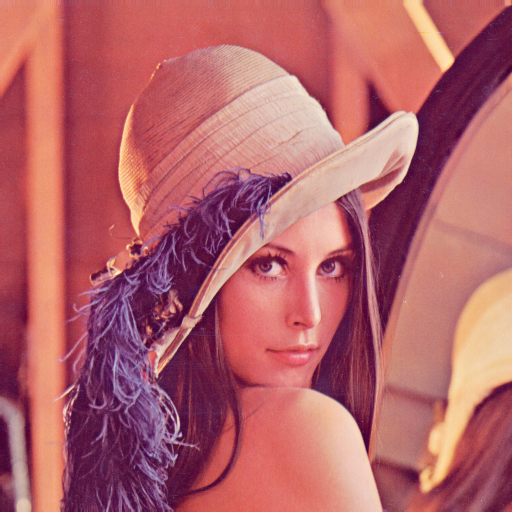
\includegraphics[width=.49\linewidth]{\detokenize{figuras/original.png}}
  }
  \subfloat[\textit{Unsharp masking}]{
    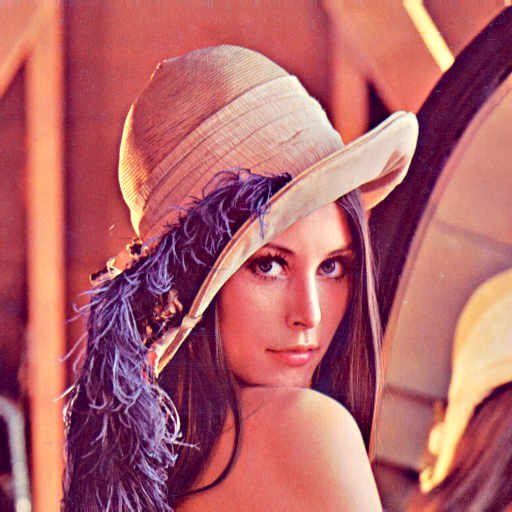
\includegraphics[width=.49\linewidth]{\detokenize{figuras/unsharpmask.png}}
    \label{fig:unsharp}
  }
 \end{center}
 \caption[A imagem original, já em escala de cinza, foi realçada utilizando o método \textit{unsharp masking}.]{A imagem original, já em escala de cinza, foi realçada utilizando o método \textit{unsharp masking}. \textit{Fonte:~Elaborado pela autora.}}
 \label{fig:pre-sharp}
\end{figure}

% Uma variação do \textit{Unsharp Mask} é uma versão adaptativa apresentada por \cite{Polesel2000}. Essa solução pretende reduzir a sensibilidade a ruido e também evitar a adição de artefatos, com o objetivo de enfatizar os detalhes que contém contraste médio e sem aplicar sharpening em áreas suaves. O resultado disso é uma imagem com maior dinâmica em áreas de detalhe e sem mudança em áreas uniformes. Para classificar uma dada região entre essas três classes (alto, médio e nenhum detalhe) foi calculado a variância local de um bloco 3x3 pixels. Esse algoritmo utiliza dois filtros direcionais com coeficientes atualizados por uma estratégia de adaptação de Gauss-Newton.

Um exemplo clássico de utilização de realce, é para compensar a variação de iluminação em diversas imagens. Em \citeonline{Gross2003}, os autores propuseram um algoritmo para o reconhecimento de faces invariante à iluminação. Eles ressaltam que, desconsiderando a variação da posição, a iluminação é o fator de maior impacto na aparência das faces. A luz varia durante o dia, entre um dia e outro, e entre diferentes ambientes. Isso afeta o conjunto de imagens a ser analisado, que passa a conter imagens com diferentes constrastes, o que pode acentuar ou diminuir certas características faciais.

O constraste é a diferença de intensidade entre os níveis de maior e menor intensidade na imagem. Imagens com baixa resolução podem ser geradas a partir de uma iluminação pobre ou outros problemas com a captura. Dessa forma, o processo de ``esticar'' o contraste expande os níveis de intensidade da imagem \cite{Gonzalez2007}.

É possível aumentar o contraste de uma imagem ao manipular o seu histograma $h$, que pode ser definido como
\begin{equation*}
h(i_k) = n_k,
\end{equation*}
\noindent onde $k$ é o índice do pixel e $n_k$ é o número de pixels de intensidade $i_k$. Ou seja, o histograma é uma representação da frequência de cada intensidade na imagem. Ao observar os histogramas de diferentes imagens, é possível notar que imagens com alto contraste possuem um histograma com níveis próximos a uma distribuição uniforme. Isso permite que certas operações, como a equalização de histograma, obtenham o melhor contraste de uma imagem. Essa operação é caracterizada pela máxima variância do histograma e pode ser definida como
\begin{equation}
s_k = T(i_k) = \frac{L-1}{MN} \sum_{j=0}^{k}n_j,
\end{equation}
\noindent onde $L$ é o número de intensidades e $MN$ as dimensões da imagem. A imagem de saída é obtida ao mapear cada pixel de intensidade $i_k$ em um nível $s_k$, com $i$ entre $[0,L-1]$, sendo $i = 0$ um pixel preto e $i = L-1$, branco \cite{Gonzalez2007}.

\enlargethispage{\baselineskip}
%-------------------------------------------------------------------------------% \subsection{Restauração}
% Ao contrário do realce, a etapa da restauração é objetiva. Também procura melhorar os aspectos visuais de uma imagem, mas com base em modelos probabilísticos de degradação de imagens. Dessa forma, tendo-se um modelo de degradação, procura-se recuperar a imagem original \cite{Gonzalez2007}. Mas um problema comum em algoritmos de remoção de ruído é que alguns detalhes, como textura, irão sofrer alta suavização.
%
% O objetivo dos algoritmos de remoção de ruído é recuperar a imagem original. Assim o modelo estatístico da imagem natural é crucial para a remoção de ruído. O tipo mais simples de ruído  é o aditivo, que pode ser caracterizado como
% \begin{equation*}
% p = p_0 + n,
% \end{equation*}
% \noindent onde $p_0$ é o valor real do pixel e $n$ é a perturbação de ruído naquele pixel.
%
% % A maneira mais simples de modelar o efeito de ruído em uma imagem digital é adicionar um ruído branco gaussiano, com média zero e variância $\sigma^2$.
%
% Um algoritmo alternativo para remoção de ruído é o de médias não locais. Isso porque pixels similares não necessariamente estão próximos em suas coordenadas cartesianas, assim, informações não locais podem ser utilizadas na redução de ruído. De acordo com \citeonline{Buades2005}, dada uma imagem ruidosa $v = {v(i) | i \in I}$, o valor estimado é calculado como uma média ponderada de todos os pixels em uma mesma imagem com
% \begin{equation*}
% v(i)= \sum_{j \in I} w(i, j)v(j),
% \end{equation*}
% \noindent onde os pesos $w(i, j)$ dependem da similaridade entre pixels.

%-------------------------------------------------------------------------------
\subsection{Quantização}
\label{sec:quantizacao}

Muitos métodos de extração de características são preparados para receber imagens de entrada em escala de cinza ou em apenas um canal de cor. Se existir a necessidade de utilizar a imagem RGB, as características são extraídas para cada canal de cor separadamente e posteriormente são concatenadas. Isso ocorre porque a complexidade de lidar com um pixel representado em três dimensões é muito maior do que em apenas uma dimensão. Assim, os métodos de quantização visam, de alguma forma, reduzir os canais de cores ($2^{3} \times 3 = 24$ bits) em apenas um ($2^{3} \times 1 = 8$ bits). \citeonline{Kanan2012} demonstraram que os métodos para a conversão de uma imagem colorida para escala de cinza influenciam a performance no reconhecimento de imagens. Eles também salientam que o método utilizado deveria estar claramente descrito nas publicações da área. Os métodos de conversão para escala de cinza utilizados nessa dissertação foram escolhidos com base em \citeonline{Kanan2012}: \emph{Gleam} e as versões corrigidas por \textit{gamma} de \emph{Intensidade} e \emph{Luminância}: \emph{Intensidade'} e \emph{Luminância'}. A operação \textit{gamma} utilizada $z' = z^{1/2.2}$ é a padrão. Os métodos de conversão para escala de cinza, utilizados nesta pesquisa, são descritos a seguir.

\begin{description}
\item [Intensidade:] consiste em computar a média entre os canais RGB da imagem a partir de
\begin{equation*}
	Q_{Intensidade} = \frac{1}{3}(R + G + B),
\end{equation*}
\noindent e então realizar a correção por \textit{gamma}, obtendo assim o método \emph{Intensidade'}.

\item [Gleam:] ao corrigir por \textit{gamma} cada canal antes de realizar a combinação linear, tem-se o método:
\begin{equation*}
	Q_{Gleam} = \frac{1}{3}(R' + G' + B'),
\end{equation*}
\noindent onde $R'$, $G'$ e $B'$ são os canais R, G e B corrigidos por \textit{gamma}.

\item [Luminância:] computa uma soma ponderada dos canais de cor. Esse método foi desenvolvido para levar em conta a percepção visual humana. O olho humano percebe verde melhor que vermelho, e vermelho melhor que azul:
\begin{equation*}
	Q_{\text{Luminância}} = 0.299R + 0.587G + 0.114B,
\end{equation*}
\noindent e então realizar a correção por \textit{gamma}, obtendo assim o método \emph{Luminância'}.

\item [Luma:]  similar ao anterior, utilizado nas televisões de alta definição:
\begin{equation*}
	Q_{Luma} = 0.2126R' + 0.7152G' + 0.0722B',
\end{equation*}
\noindent onde $R'$, $G'$ e $B'$ são os canais R, G e B corrigidos por \textit{gamma}.

\item [\sigla{MSB}{\textit{Most Significant Bits}}:] ao invés de realizar uma combinação linear dos canais de cores, ordena os bits dos canais coloridos em um único canal. Computa quantos bits de cada canal de cor contribuem para a imagem final e extrai os bits do código binário dos canais originais \cite{Ponti-Jr2013}.

\end{description}

A Figura \ref{fig:quantizacao} apresenta a conversão na escala de cinza obtida com o uso desses métodos. A análise específica da aplicação de cada método é discutida no Capítulo \ref{cap:quantization}.


\begin{figure}[!htbp]
 \begin{center}
\subfloat[Original]{
  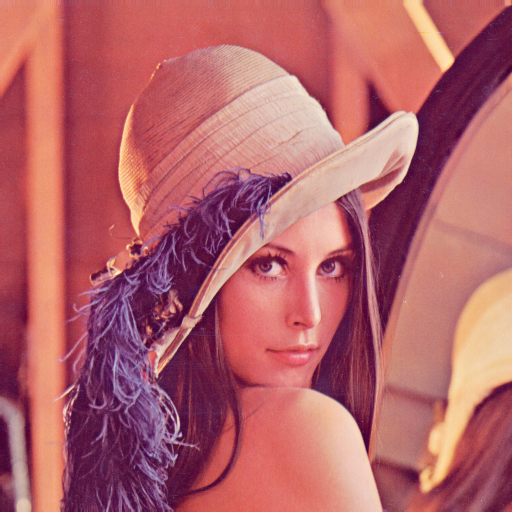
\includegraphics[width=.3\linewidth]{\detokenize{figuras/quantizacao/Lenna.png}}
}
\subfloat[Intensidade]{
  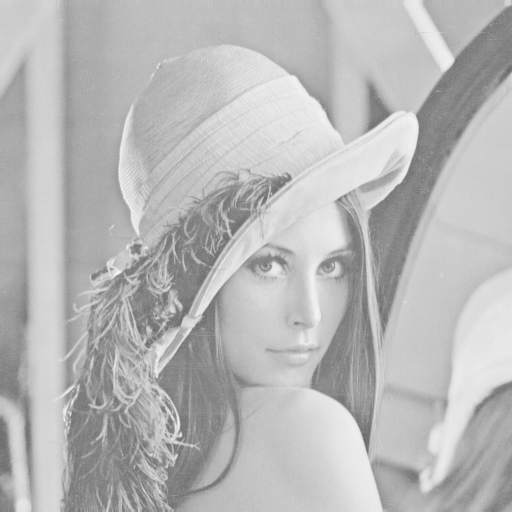
\includegraphics[width=.3\linewidth]{\detokenize{figuras/quantizacao/Intensity_gray.png}}
  \label{fig:intensidade}
}
\subfloat[Gleam]{
  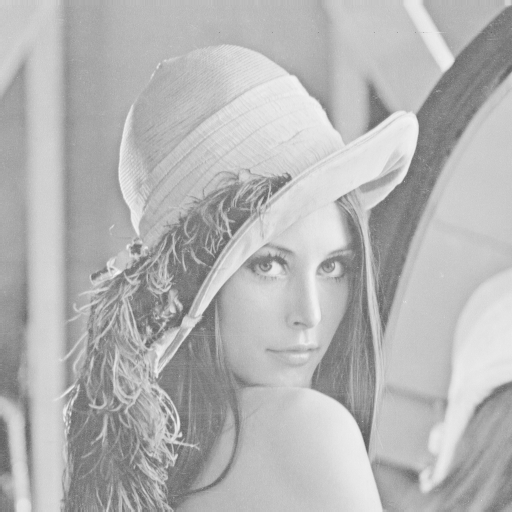
\includegraphics[width=.3\linewidth]{\detokenize{figuras/quantizacao/Gleam_gray.png}}
  \label{fig:gleam}
}
\newline
\subfloat[Luminância]{
  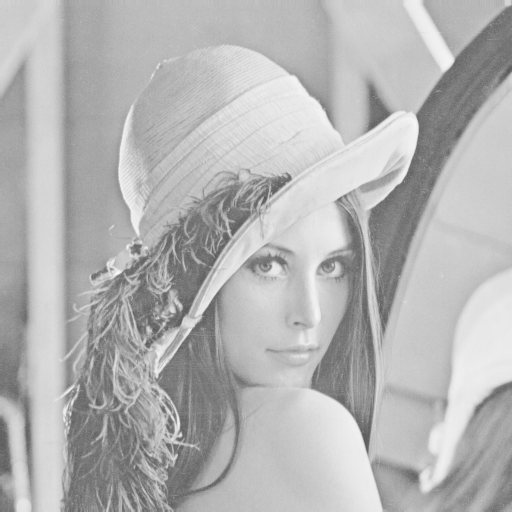
\includegraphics[width=.3\linewidth]{\detokenize{figuras/quantizacao/Luminance_gray.png}}
  \label{fig:Luminance}
}
\subfloat[Luma]{
  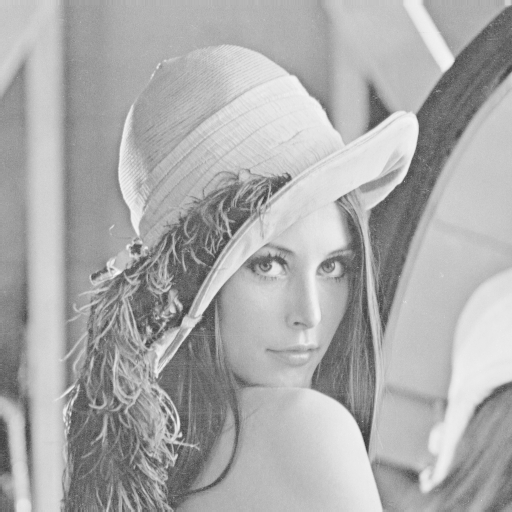
\includegraphics[width=.3\linewidth]{\detokenize{figuras/quantizacao/Luma_gray.png}}
  \label{fig:luma}
}
\subfloat[MSB]{
  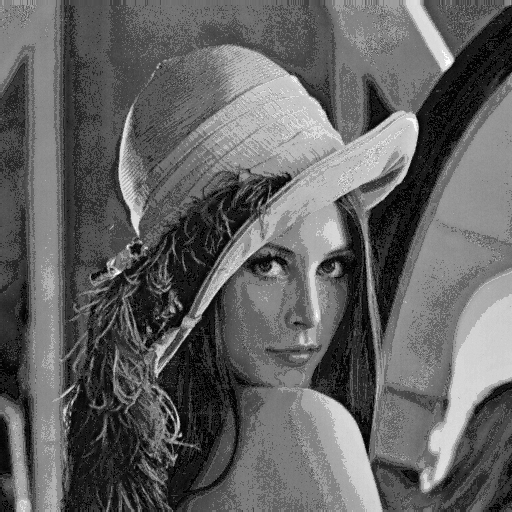
\includegraphics[width=.3\linewidth]{\detokenize{figuras/quantizacao/MSB_gray.png}}
  \label{fig:msb}
}
 \end{center}
 \caption[Conversão para a escala de cinza com os métodos utilizados nessa pesquisa. O método MSB resulta em uma imagem com 8 bits (64 cores) e os outros em 256 cores.]{Conversão para a escala de cinza com os métodos utilizados nessa pesquisa. O método MSB resulta em uma imagem com 8 bits (64 cores) e os outros em 256 cores. \textit{Fonte:~Elaborado pela autora.}}
 \label{fig:quantizacao}
\end{figure}

\meutodo{Porque o MSB resultou em 64 cores e não 256?}

%--------------------------------------------------------------------------------
% \subsection{Reconstrução}

% \meutodo{Seção reconstrução? fisher faces}

% Fisherfaces é utilizado para reconhecimento de faces, reconstrói faces para a posterior classificação. No contexto deste estudo, esse método pode ser utilizado para gerar novas imagens a partir das já existentes como para auxiliar no problema do desbalanceamento de classes (descrito na Seção \ref{cap:desbalanceamento}). Especificamente para a sobreamostragem do conjunto de dados de entrada.

% Calcula os autovetores de todas as imagens de treinamento. Seleciona as com maior valor de autovalores.

% Primeiramente é realizado o cálculo do PCA para reduzir a dimensão $N-c$ (onde $N$ é o número de imagens e $c$ o número de classes) e então aplicado o FLD (\textit{Fisher Linear Discriminant}) para reduzir a $c-1$. A reconstrução tende a desconsiderar porções da imagem que não a discriminam. Considera cada pixel em uma imagem como uma coordenada.

% Esse método calcula a matriz de covariância das imagens originais e sua matriz de transformação $W$ com colunas ortonormais. Em seguida, tenta-se encontrar a melhor matriz $W$. Essa matriz é selecionada pela maximização da razão entre as matrizes de espalhamento intra e inter~\cite{Belhumeur1997}. Isso é expresso pela equação:

% \begin{equation}
% W = W_{FLD}^{T} W_{PCA}^{T}.
% \end{equation}

% As matrizes de transformação que projetam a matriz original é então dada por:

% \begin{eqnarray}
%     W_{PCA} &=& \operatorname{arg\,max}_{W} |W^T S_T W| \\
%     W_{FLD} &=& \operatorname{arg\,max}_{W} \frac{|W^T W_{PCA}^T S_{B} W_{PCA} W|}{|W^T W_{PCA}^T S_{W} W_{PCA} W|}
% \end{eqnarray}

% Essa matriz $W$ é portanto a reconstrução da imagem original.

%--------------------------------------------------------------------------------
\section{Extração de características}
\label{sec:extracao}

O objetivo da extração de características é descrever as informações visuais relevantes em um vetor de características. Esse vetor pode ser utilizado como entrada para um algoritmo de classificação de padrões. Por exemplo, em aplicações que envolvem a classificação de algas, uma informação muito importante para a discriminação entre classes é a forma \cite{Borges2013}. Características, como essa, devem salientar as diferenças entre imagens de classes distintas e suavizar possíveis diferenças de imagens da mesma classe. Algumas características, segundo~\citeonline{Gonzalez2007}, são:

\begin{description}
\item [Textura:] na sua descrição estatística, possui propriedades como: suavidade, aspereza e uniformidade. Um exemplo de medida para descrever a textura é a entropia.
\item [Forma:] representa os objetos em termos de suas características externas, como por exemplo, a medida da curvatura.
\item [Cor:] considera a distribuição espacial de cores na imagem. O histograma de uma imagem pode descrever essa configuração de forma global.
\end{description}

Exemplos de métodos conhecidos capazes de descrever outras características são: histogramas de orientação de gradiente~\cite{Wang2009}, descritores de Fourier, métodos baseados na detecção de SUSAN~\cite{Smith1997}, Harris-Affine~\cite{Han2005b} e diferença de Gaussianas~\cite{Lowe2004a}. Os descritores utilizados no desenvolvimento desta pesquisa para a obtenção dos resultados dos Capítulos \ref{cap:resultados-quantizacao} e \ref{cap:resultados-geracao} estão abaixo descritos.

\begin{description}
\item[\sigla{GCH}{\textit{Global Color Histogram}}:] calcula o histograma global dos níveis de intensidade da imagem. É a alternativa mais simples para representar as informações de uma imagem~\cite{Gonzalez2007}. Produz um vetor de $N$ dimensões, sendo $N$ o número de intensidades.

\item[\sigla{CCV}{\textit{Color Coherence Vector}}:] captura informações sobre como as cores são organizadas em regiões conectadas, de acordo com um \textit{threshold}. Classifica os pixels da imagem em coerentes e incoerentes, computa os respectivos histogramas e os concatena \cite{ccv}. Dessa forma, o vetor de características produzido possui $2N$ dimensões.

O vetor de coerência de cor armazena o número de pixels coerentes e de incoerentes para cada cor. Pixels coerentes fazem parte de uma região contígua enquanto incoerentes não. Seu funcionamento pode ser resumido nos seguintes passos:

\begin{enumerate}
  \item Borra levemente a imagem ao substituir os pixels pela média do pixel e seus oito vizinhos;
  \item Discretiza o espaço de cor de forma que a imagem contenha apenas $n$ cores distintas;
  \item Classifica os pixels entre coerentes e incoerentes: se o tamanho do seu componente conectado for maior ou igual um \textit{threshold} é coerente; caso contrário, incoerente;
  \item Computa dois histogramas:
  \begin{itemize}
    \item Histograma de pixels coerentes;
    \item Histograma de pixels incoerentes.
  \end{itemize}
  \item Concatena os histogramas.
\end{enumerate}

\item[\sigla{BIC}{\textit{Border-interior classification}}:] computa dois histogramas, um para pixels definidos como borda e outro como interior. Se um pixel possuir a mesma cor que seus vizinhos, é pixel de interior; caso contrário, será pixel de borda. Os histogramas são concatenados, gerando um vetor de $2N$ dimensões \cite{bic}. Para computar tal vetor, as operações realizadas são:

\begin{enumerate}
  \item Os pixels são classificados entre borda e interior:
  \begin{itemize}
    \item \emph{Borda:} se está na borda da imagem ou se ao menos um dos seus quatro vizinhos tem uma cor diferente do que o próprio pixel;
    \item \emph{Interior:} se seus quatro vizinhos possuem a mesma cor.
  \end{itemize}
  \item Computa dois histogramas:
  \begin{itemize}
    \item Histograma dos pixels classificados como borda;
    \item Histograma dos pixels classificados como interior.
  \end{itemize}
  \item Concatena os histogramas.
\end{enumerate}

\item[\sigla{ACC}{\textit{Auto Color Correlogram}}:] captura a correlação espacial entre cores idênticas. Para tal, computa a probabilidade de encontrar dois pixels com a mesma cor, a uma distância $d$ um do outro \cite{acc}. O vector resultante consiste na concatenação dos auto-correlogramas, um para cada distância. Neste estudo, são consideradas quatro distâncias: 1, 3, 5 e 7; resultando em um vetor com $4N$ características.

\item[Haralick-6:] descreve a textura das imagens, ou seja, diferenças locais em níveis de intensidade~\cite{Haralick1973}. O vetor resultante possui seis dimensões que representam as seguintes características:

\begin{enumerate}
  \item \emph{Probabilidade máxima:} maior resposta na matriz de co-ocorrência. Intervalo:~$[0,1]$;
  \item \emph{Correlação:} descreve as correlações entre as linhas e colunas da matrix.\\ Intervalo:~$[-1,1]$;
  \item \emph{Contraste:} mede as variações locais dos níveis de cinza da matriz.\\ Intervalo:~$[0, (colors-1)^2]$;
  \item \emph{Uniformidade:} soma dos elementos quadrados. Também conhecido como energia ou segundo momento angular. Intervalo:~$[0,1]$;
  \item \emph{Homogeneidade:} mede a proximidade da distribuição dos elementos em relação à diagonal. Intervalo:~$[0,1]$;
  \item \emph{Entropia:} descreve a aleatoriedade. Intervalo:~$[0, 2*log_2 colors]$.
\end{enumerate}

\item [\sigla{HOG}{\textit{Histogram of oriented gradients}}:] calcula a frequência da ocorrência da orientação dos gradientes em janelas na imagem \cite{Dalal2005}:

\begin{enumerate}
  \item Divide a janela da imagem em células;
  \item Computa os gradientes;
  \item Cada pixel calcula uma ponderação para um canal do histograma de orientação de bordas baseado na orientação do gradiente do elemento em que está centrado. Esses valores são acumulados em \textit{bins} sobre as regiões espaciais de células e formam o histograma;
  \item As ocorrências são interpoladas bilinearmente entre os centros de vizinhança do \textit{bin} em orientação e posição;
  \item Normaliza o contraste dos blocos da janela que se sobrepõem. Dessa forma cada célula é normalizada em relação a diferentes blocos;
  \item Concatena os histogramas de todas as células.
\end{enumerate}

\item [\sigla{LBP}{\textit{Local Binary Patterns}} utilizando padrões uniformes:] baseia-se em reconhecer que padrões de textura uniformes são propriedades fundamentais da textura local da imagem. O histograma da sua ocorrência provou-se ser um bom extrator de características. Computa um histograma de ocorrência dos padrões locais binários em uma vizinhança da imagem, detectando micro-estruturas cuja distribuição é estimada pelo histograma \cite{Ojala2002}:

\begin{enumerate}
  \item Divide a janela da imagem em células;
  \item Compara cada pixel em uma célula com seus vizinhos. Esse passo resulta em um código binário de oito dígitos;
  \item Computa o histograma da célula;
  \item Normaliza o histograma;
  \item Concatena os histogramas de todas as células.
\end{enumerate}

\end{description}

% %-------------------------------------------------------------------------------\section{Características latentes}
% \label{sec:latentes}
%
% Assim como o método de quantização se mostrou relevante na classificação, nesta dissertação são estudados diversos métodos de pré-processamento de imagens, como filtros de borramento e deconvolução, com o objetivo de obter imagens processadas que sejam mais bem caracterizadas para a etapa de classificação (ou seja, aumentando a variância entre as classes, sem aumentar a variância intra-classe). O enfoque está em como realçar determinadas características, como por exemplo cor, textura e forma. A esses atributos pode-se dar o nome de características latentes, não visíveis na imagem original. Identificar e realçar tais características é objetivo deste estudo. Essa abordagem se diferencia das técnicas multi-resolução, pois não pretende encontrar apenas características em versões de diferentes resoluções (convoluídas com filtros passa-baixa), e sim também em versões deconvoluídas ou transformadas por outros operadores.
%
% Se uma das principais características que diferenciam classes de uma certa base utiliza a sua forma, é possível utilizar o método de diferença de Gaussianas para ressaltá-la.
% % Considerando, por exemplo, uma série de imagens filtradas por um filtro Gaussiano definido como $f_1(x,y) = G_{\sigma}(f(x,y))$.
% O método DoG (\textit{Difference of Gaussians}) se baseia na diferença entre duas imagens filtradas. A operação comumente é feita usando $\sigma = \sqrt{2}$ e sua definição para dois níveis de filtragem é definida por
% \begin{eqnarray*}
%          f_1(x,y) &=& G_{\sigma}(f(x,y)) \\
%          f_2(x,y) &=& G_{\sigma}(f_1(x,y)) \\
%          DoG_1(x,y,\sigma) &=& f_2 - f_1
% \end{eqnarray*}
%
% A Figura~\ref{fig:caracteristicas} demonstra uma possível execução de filtragem e restauração seguida pela detecção de bordas por DoG, aplicadas em uma base de imagens de algas verdes.
%
% \renewcommand{\tabcolsep}{0.0cm}
% \begin{figure}[htbp]
%  \begin{center}
% \subfloat{
%   \centering
%   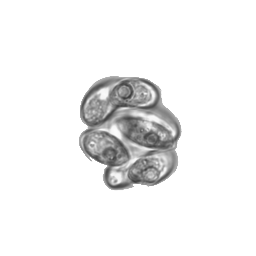
\includegraphics[width=\linewidth]{\detokenize{figuras/alga_05b.png}}
%   \caption{}}
%   \label{fig:algaa}
%
% \subfloat{
%   \centering
%   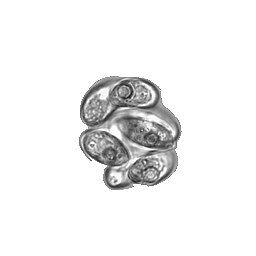
\includegraphics[width=\linewidth]{\detokenize{figuras/alga_05c.png}}
%   \caption{}}
%   \label{fig:algab}
%
% \subfloat{
%   \centering
%     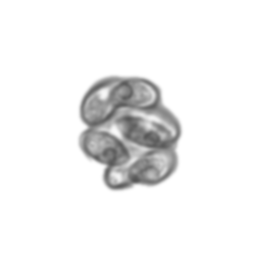
\includegraphics[width=\linewidth]{\detokenize{figuras/alga_05d.png}}
%   \caption{}}
%   \label{fig:algac}
%
% \subfloat{
%   \centering
%   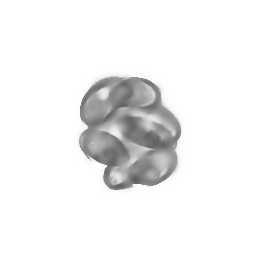
\includegraphics[width=\linewidth]{\detokenize{figuras/alga_05e.png}}
%   \caption{}}
%   \label{fig:algad}
%
% \subfloat{
%   \centering
%   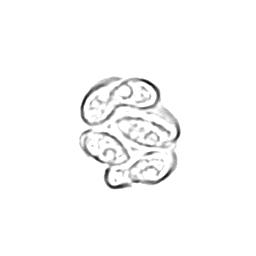
\includegraphics[width=\linewidth]{\detokenize{figuras/alga_05ba.png}}
%   \caption{}}
%   \label{fig:algae}
%
% \subfloat{
%   \centering
%   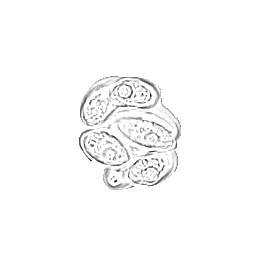
\includegraphics[width=\linewidth]{\detokenize{figuras/alga_05ca.png}}
%   \caption{}}
%   \label{fig:algaf}
%
% \subfloat{
%   \centering
%   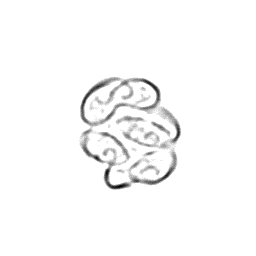
\includegraphics[width=\linewidth]{\detokenize{figuras/alga_05da.png}}
%   \caption{}}
%   \label{fig:algag}
%
% \subfloat{
%   \centering
%   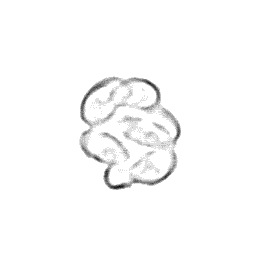
\includegraphics[width=\linewidth]{\detokenize{figuras/alga_05ea.png}}
%   \caption{}}
%   \label{fig:algah}
%
% \subfloat{
%   \centering
%   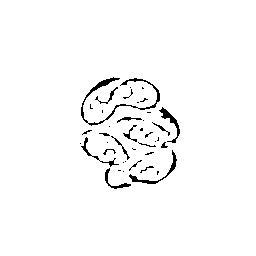
\includegraphics[width=\linewidth]{\detokenize{figuras/alga_05bb.png}}
%   \caption{}}
%   \label{fig:algai}
%
% \subfloat{
%   \centering
%   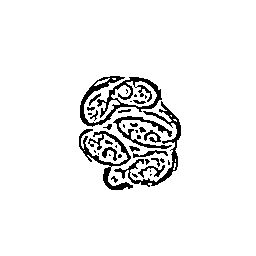
\includegraphics[width=\linewidth]{\detokenize{figuras/alga_05cb.png}}
%   \caption{}}
%   \label{fig:algaj}
%
% \subfloat{
%   \centering
%   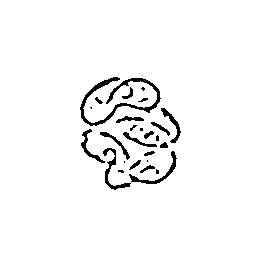
\includegraphics[width=\linewidth]{\detokenize{figuras/alga_05db.png}}
%   \caption{}}
%   \label{fig:algak}
%
% \subfloat{
%   \centering
%   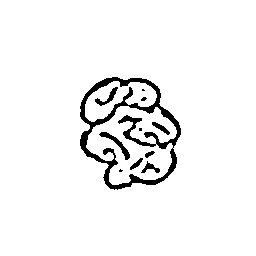
\includegraphics[width=\linewidth]{\detokenize{figuras/alga_05eb.png}}
%   \caption{}}
%   \label{fig:algal}
%
%
%  \caption[Características latentes de algas verdes.]{Características latentes de algas verdes. A primeira imagem (a) é uma imagem original segmentada de alga. As próximas colunas são imagens resultantes da deconvolução da imagem (coluna 2), filtragem Gaussiana (coluna 3) e filtragem Gaussiana seletiva (coluna 4). A primeira linha mostra versões diferentes de imagens de algas, a segunda linha exibe imagens resultantes da diferença de Gaussianas, e a terceira linha demonstra imagens binárias obtidas por limiarização das imagens contidas na segunda linha). \textit{Fonte:~Elaborado pela autora.}}
%  \label{fig:caracteristicas}
%  \end{center}
% \end{figure}
% \renewcommand{\tabcolsep}{0.25cm}
%
% A imagem \ref{fig:algaa} é uma imagem original segmentada de alga. As próximas colunas são imagens resultantes da deconvolução da imagem (coluna 2), filtragem Gaussiana (coluna 3) e filtragem Gaussiana seletiva (coluna 4). As modificações apresentadas na primeira linha geram informações em diferentes planos axiais da imagem de microscopia. Imagens na segunda coluna representam uma versão deconvoluída das imagens originais, ressaltando a textura na superfície das algas, resultantes da diferença de Gaussianas. Já a terceira linha demonstra imagens binárias obtidas por limiarização das imagens da segunda linha, realçando as características da base da célula.
%
% Acredita-se que ao manipular as imagens através de técnicas de pré-processamento, pode-se gerar imagens artificiais com características latentes realçadas, melhorando a extração de características.
%--------------------------------------------------------------------------------
% \section{Deep learning}
% \label{sec:deeplearning}
%
% % O cérebro humano está em constante aprendizado. Suponha que uma determinada pessoa nunca tenha visto um \textit{drone}. Ela então lê uma pesquisa recente sobre esses veículos aéreos contendo uma foto de um exemplar. Enquanto isso, essa tecnologia acaba se tornando mais acessível e surgem várias publicações na mídia sobre eles. Após tê-los visto algumas vezes, essa pessoa será capaz de reconhecer visualmente um \textit{drone} em imagens, vídeos e até mesmo de diferentes cores e tamanhos em relação às imagens que tinha visto anteriormente.
%
% % Dessa forma, ao se expor a alguns padrões, ela aprendeu a reconhecê-los. Essa capacidade dos sistemas de aprendizado (como o cérebro humano) de reconhecer novos padrões está diretamente relacionada com a capacidade de generalização. Nesse sentido, generalizar é como ter visto um \textit{drone} de cor preta medindo 1 metro e ao ver um outro de cor branca de 20 metros, classificá-lo como sendo um \textit{drone} também, porque aprendeu as principais características.
%
% A habilidade humana de reconhecimento de padrões em imagens é surpreendente. Os algoritmos de aprendizado de máquina e de reconhecimento de padrões tentam habilitar os computadores a aprender, baseando-se no modelo de aprendizado de seres humanos \cite{thesisDeep}. Considerando que existem milhões de neurônios em cada córtex visual e que o cérebro humano é composto por cinco desses córtex que evoluíram durante milhões de anos, pode-se afirmar que a tarefa de algoritmos de reconhecimento de padrões em imagens não é simples \cite{neuralNielsen}.
%
% A capacidade humana de reconhecer novos padrões está diretamente relacionada com a capacidade de generalização, que para tal, utiliza hierarquias \cite{thesisDeep}. Nessa linha, o aprendizado profundo ou \textit{deep learning} é caracterizado por explorar o aprendizado ao simular o funcionamento do cérebro humano. Essa área está diretamente relacionada com aprendizado de máquina e inteligência artificial e lida com o aprendizado através de múltiplas camadas.
%
% Explicitar quais são as regras para aprender um determinado conceito pode se tornar impossível. No caso de um avião, por exemplo, ``voar'' pode ser uma regra decomposta em ``possuir largura maior que altura'' e ``ser aerodinâmico''. Essas subdivisões geram múltiplos níveis que possuem maior complexidade e abstração, de maneira similar ao aprendizado por camadas. Uma rede neural artificial utiliza imagens como treinamento para automaticamente inferir quais são as regras para o reconhecimento. São chamadas de redes neurais profundas ou \textit{deep neural networks} as redes que possuem uma estrutura de muitas camadas -- duas ou mais ocultas \cite{neuralNielsen}. Assim, dada uma imagem como entrada, o problema é subdividido em problemas mais simples de serem resolvidos, podendo chegar ao nível de pixels isolados.
%
% As redes neurais artificiais consistem em um método para solucionar problemas de forma a simular o comportamento do cérebro humano. Ao tentar uma determinada solução e errar, essas redes aprendem e podem tentar novamente. Ou seja, adquirem conhecimento através da experiência. Elas contém neurônios de entrada, ocultos e de saída. Aprender nesse contexto significa encontrar os pesos que fazem com que a rede neural exiba o comportamento esperado \cite{Schmidhuber2014}.
%
% % Hubel e Wiesel publicaram em 1962 uma pesquisa relacionada ao estudo do córtex visual primário de gatos. Eles identificaram células simples, similares aos layers de bancos de filtros de uma ConvNet e células complexas similares aos layers de pooling.
%
% A simulação desse modelo inspirado biologicamente utilizada hoje é de \citeonline{lecun1998} e chama-se Rede Neural de Convolução (CNN ou ConvNet). Eles simplificaram tal arquitetura para utilizar um algoritmo de retropropagação para o treino. Desde então, essas redes vêm sendo utilizadas para detecção, reconhecimento, restauração, remoção de ruído e segmentação de imagens e vídeos, além de sua aplicação em áudio. Um exemplo de utilização dessa rede inspirada no modelo de LeCun foi desenvolvida pela empresa Google, com o objetivo de detectar faces e placas de carros para proteger a privacidade nas imagens de StreetView \cite{google09}.
%
% % \meutodo{Figura da visualização do resultado dos filtros}
%
% Apesar de redes profundas representarem o estado da arte em visão computacional, um bom entendimento das suas propriedades ainda está faltando. Alguns artigos recentes como \citeonline{Mahendran2014}, \citeonline{Zeiler2011} \citeonline{Zeiler2013} e \citeonline{Simonyan2013} introduzem técnicas utilizadas para analisar o comportamento e operações internas dessas redes ao visualizá-las. Esta pesquisa situa-se nesse viés, ao analisar as características latentes extraídas por uma rede neural de convolução.
%
% Para o uso em bases desbalanceadas, as imagens utilizadas para o rebalanceamento de forma visual podem ser geradas após o estudo das características latentes, encontradas no treinamento da classe minoritária em uma CNN. Essas características também podem ser realçadas de forma a melhorar a classificação de imagens.
%
% %--------------------------------------------------------------------------------
% \subsection{Redes de convolução}
% % As redes de convolução são modelos que podem aprender características, e são compostas por diversas camadas.
%
% São um tipo de rede neural que utiliza uma operação chamada de convolução, previamente descrita na Seção \ref{sec:convolucao}. Pode ser entendida como sendo várias multiplições de um filtro espacial pela imagem de entrada, resultando em um mapa de características ativadas. Esse filtro é um vetor de parâmetros capaz de aprender. Cada imagem possui seu conjunto de mapas de características, mas os filtros são comuns a todas as imagens. Dependendo dos valores do filtro, as características ativadas são diferentes. Nesse contexto, a camada de convolução consiste em muitas aplicações de convolução em paralelo, dado que um filtro é capaz de extrair apenas um tipo de característica \cite{Bengio-et-al-2014-Book}.
%
% Basicamente, uma CNN é uma arquitetura que pode aprender características invariantes. Com múltiplas camadas, ela pode aprender multiníveis de características \cite{lecun2010}. Ou seja, permite ao computador criar conceitos complexos a partir de conceitos simples. Como o conceito de \textit{deep learning} enfatiza o uso de variáveis latentes, sugere que algoritmo de treinamento pode inventar os conceitos que precisa para representar determinada base de dados \cite{Bengio-et-al-2014-Book}.
%
% Cada camada é composta de três estágios~\citeonline{lecun2010}, representados na Figura~\ref{fig:cnn}:
%
% \begin{description}
% \item [Estágio de convolução:] várias convoluções em paralelo para produzir um conjunto de ativações pré-sinápticas;
% \item [Estágio de detecção:] função de ativação, como a unidade linear retificada ou a sigmoide;
% \item [Estágio de \textit{pooling}:] retorna uma representação invariante a pequenas translações da entrada. Um exemplo é utilizar o valor máximo entre vizinhos (conhecido como \textit{max-pooling}). %Essa operação é de pós-processamento.
% \end{description}
% \begin{figure}[htbp]
%  \begin{center}
%    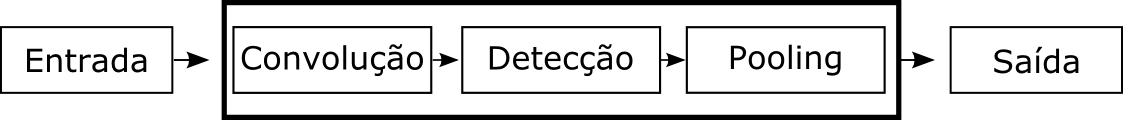
\includegraphics[width=1\linewidth]{figuras/convlayer.png}
%  \end{center}
%  \caption[Componentes típicos de uma camada de uma rede neural de convolução.]{Componentes típicos de uma camada de uma rede neural de convolução. Nessa terminologia a rede possui camadas complexas que possuem estágios \cite{Bengio-et-al-2014-Book}. \textit{Fonte:~Elaborado pela autora.}}
%  \label{fig:cnn}
% \end{figure}
%
% % Normalmente o kernel é muito menor que a imagem, o que resulta em menos parâmetros a serem armazenados, o que reduz o uso de memória e melhorando a eficiência.
% % Cada membro do kernel é usado em todas as posições da entrada, provocando invariância a translação. Por isso só é interessante usar uma camada de convolução quando o que é para ser aprendido é invariante a translação. Em alguns casos, como detecção de faces, não é tão interessante -- deve procurar a sombrancelha em cima e o queixo embaixo.
% % Ao processar dados temporais, o resultado de séries de convoluções produzem uma espécie de timeline ou mapa que mostra quando e aonde características diferentes aparecem na entrada.
% % Não é invariante a escala e a rotação.
% % É possível aprender invariâncias utilizando pool sobre as saídas das convoluções. Essa etapa sumiariza as respostas sobre uma vizinhança inteira, assim é possível utiilizar menos unidades de pooling do que unidades de detecção, resultando em um downsampling.
% % Uma característica essencial na implementação é o método escolhido para adição de zeros nas bordas da imagem. Sem isso o tamanho da representação diminui a kernel-1 a cada camada.
% % % Se pensarmos na convolução como uma multiplicação por uma matriz esparsa que possui cada elemento do kernel copiado várias vezes, a multiplicação da imagem de entrada pela transposta dessa matriz permite backpropagar os erros.
% % Para termos aprendizagem, é preciso computar o gradiente a respeito do kernal, dado o gradiente das saídas.
%
% De acordo com \citeonline{Bengio-et-al-2014-Book}, durante a propagação são realizadas as convoluções e propagadas pelo resto da rede para então computar uma função de perda, que mede quão bem o sistema de aprendizado funcionou para cada exemplo. Na retropropagação, recebe-se um gradiente para atualizar os pesos. O gradiente descendente estocástico atualiza o sistema de aprendizagem com base no erro medido para um único exemplo. Apesar de a convergência ser mais ruidosa do que calcular a média sobre todos os erros, diminui-se um custo constante do calculo de custo.
%
% Normalmente, o classificador é a última camada totalmente conectada, que computa o produto de um vetor de características \cite{Bengio-et-al-2014-Book}. \citeonline{Mahendran2014} reportam que as camadas inteiramente conectadas podem ser invertidas a uma imagem resultante da composição de partes similares às encontradas na imagem original, mas não idênticas. Enfatizam também que todas as camadas de convolução mantém uma representação fiel da imagem. Essa característica permite a análise de quais atributos são relevantes para o aprendizado da base de imagens, tarefa crucial para esta pesquisa.
%
%
% % % --------------------------------------------------------------------------------
% % \subsection{Redes de deconvolução}
%
% \citeonline{Zeiler2011} propuseram uma rede de deconvolução para a visualização das camadas, que pode ser vista como o caminho inverso de uma rede de convolução. Dessa forma, ao invés de mapear pixels em características, faz-se o contrário, permitindo a construção não supervisionada de representação de imagens hierárquicas, que podem, por exemplo, ser usadas para redução de ruído \cite{Zeiler2013}. Tenta gerar o sinal de entrada dada a soma das convoluções dos mapas de características com os filtros aprendidos. Apesar de destacar que, dado o mapa de características latentes, é possível sintetizar uma imagem, o artigo de \citeonline{Zeiler2011} não discorre sobre essa síntese.
%
%
% % Em \citeonline{Zeiler2013}, eles reverteram as computações para identificar quais pedaços das imagens eram responsáveis por certas ativações neurais. Olham sobre como certos outputs são obtidos
% % Mas nesse artigo: http://arxiv.org/pdf/1412.0035v1.pdf eles reconstroem as imagens. Dessa forma, eles mostram que as CNN retêm inforações fotograficamente precisas sobre a imagem, com diferentes graus de invariância.
% % Qual informação é preservada pela saída da rede.
% % A representação aprendida pode então ser utilizada para síntese. Em \cite{Zeiler?} um exemplo de redução de ruído é apresentado. Ao utilizar as características latentes da segunda camada para reconstruir a imagem, o ruído foi reduzido de 13.84dB para 18.01dB.
%
% % A operação de reconstrução pode ser definida como:
%
% % % \begin{equation}
% % % Ŷ_1 = (F_1)(U_(s_1))...(F_L)(U_(s_L)) = (R_l)(z_L)
% % % \end{equation}
%
% % % Com $ŷ_1$ sendo a imagem reconstruída, F a convolução, U unpool, z o mapa de características, s os switches de pooling e L o número de camadas.
%
% %--------------------------------------------------------------------------------
% \section{Máquinas de Boltzmann restritas}
% \label{sec:rbm}
%
% Uma máquina de Boltzmann restrita (RBM) é uma rede neural estocástica que treina um modelo a partir dos vetores de entrada. Ela aprende os parâmetros que definem a distribuição sobre um conjunto de observações sem retropropagação e baseando-se em energia \cite{Fischer2014}.
%
% Diferente de uma rede de Hopfield, ela agrega probabilidades e encontra a mínima energia global. Faz isso através do arrefecimento simulado (\textit{simulated annealing}), ou seja: em um primeiro momento, quando possui energia alta, aceita configurações piores; e conforme a energia é reduzida, detêm-se a uma região e a explora melhor, até o equilíbrio térmico \cite{Hinton2006}.
%
% Possuindo uma arquitetura muito mais simples que a CNN, é composta por duas camadas de neurônios: uma visível e outra oculta. Os pixels correspondem às unidades visíveis e os detectores de características às unidades ocultas. A sua restritividade se deve ao fato da falta de conectividade entre os neurônios de uma mesma camada, mas cada unidade visível é conectada a todas as unidades ocultas. Assim, a camada oculta, de detectores de características, modela a correlação entre os pixels.
%
% A aprendizagem de uma RBM começa em um estado aleatório e atualiza seus pesos até encontrar uma distribuição que esteja em equilíbrio. Essa convergência ocorre quando o erro entre os exemplos treinados -- fase positiva -- e suas reconstruções -- fase negativa -- é menor que um certo limiar. Dessa forma, a cada iteração, um novo exemplo é treinado ao repetir iterativamente esses dois estágios e atualizar seus pesos \cite{Hinton2006}.
%
% \begin{description}
% \item [Fase positiva:] fixa a camada visível e computa o valor dos neurônios ocultos. A probabilidade de um neurônio oculto ser ativado (se torne igual a 1) é dada pela função
% \begin{equation}
% p(h_j = 1) = \frac{1}{1+e^{-(b_j+\sum_{i\epsilon vis}{v_iw_{ij}})}},
% \label{eq:prob}
% \end{equation}
% \noindent onde $p(h_{j})$ é a probabilidade do neurônio $h_j$ ser ativado, utilizando uma função de ativação sigmóide, e $w_{ij}$ o peso entre a entrada $i$ e o neurônio $j$.
%
% A contribuição da fase positiva é computada para cada par de unidades $a_{ij}$, ao conferir se os dois neurônios ($x_i$ e $x_j$) estão ativados por meio de
% \begin{equation*}
% Fase_{+}(a_{ij}) = x_i . x_j
% \end{equation*}
%
% \item [Fase negativa:] a partir dos valores computados na fase positiva, os neurônios visíveis são ``reconstruídos'' ($p(v_i)$) e os ocultos novamente computados ($p(h_{j'})$) a partir da função de probabilidade da Equação \eqref{eq:prob}.
%
% % \begin{equation}
% % p(h_i = 1) = \frac{1}{1+e^{-(b_i+\sum_{j\epsilon vis}{v_jw_{ji}})}}
% % \label{eq:phi}
% % \end{equation}
%
% A contribuição da fase negativa é calculada da mesma forma que a contribuição positiva, com
% \begin{equation*}
% Fase_{-}(a_{ij}) = x_i . x_j
% \end{equation*}
%
% \item [Atualização dos pesos:] os pesos $w_{ij}$ são ajustados considerando a diferença entre os neurônios visíveis reconstruídos e os valores fornecidos de entrada inicialmente (etapa conhecida como \textit{contrastive divergence}):
% \begin{equation*}
% w_{ij} = w_{ij} + L (Fase_{+}(a_{ij}) - Fase_{-}(a_{ij})),
% \end{equation*}
% \noindent onde $L$ é a taxa de aprendizado. Quanto menor esse valor, melhor o treinamento e maior tempo até a convergência.
% \end{description}
%
%
%
% % Hinton e Seynowsky, em 1983, estenderam o modelo de Hopfield com a incorporação de dinâmica estocástica. Este modelo de rede neural passou a ser conhecido como Máquina de Boltzmann.
%
% % \begin{equation}
% % E(v,h) = - \sum{iEvisivel}{a_i v_i} - \sum{jEoculta}{b_j h_j} - \sum{i, j}{v_i h_j W_ijs}
% % \end{equation}
%
% % onde $v_i$ é o estado binário da unidade visível, $h_j$ estado binário da unidade oculta, $a_i$ e $b_j$ seus biases e $w_ij$ o peso entre eles.
% Essas redes também podem ser usadas como classificadores, ao treiná-las para modelar a relação entre a distribuição de entrada e seus respectivos rótulos \cite{Fischer2014}. Devido à capacidade das máquinas de Boltzmann restritas de aprender representações das imagens, pode-se utilizá-las para identificar se uma imagem é relevante para o aprendizado. Pode-se, por exemplo, utilizar apenas um neurônio, com a matriz de pesos representando uma memória associativa, para entender quais imagens são mais relevantes dentro de uma classe arbitrária. Dessa forma, também é possível avaliar a relevância da informação contida em uma imagem artificialmente gerada.

%--------------------------------------------------------------------------------
\section{Desbalanceamento de classes}
\label{cap:desbalanceamento}

Nesta seção é definido o problema do desbalanceamento de classes e apresentados os trabalhos relacionados que possuem duas diferentes abordagens: sobreamostragem (\textit{over-sampling}) e subamostragem (\textit{under-sampling}).

Em conjuntos de dados desbalanceados, determinadas classes possuem um número muito maior de instâncias do que outras. As classes com mais elementos são chamadas de classes majoritárias, e as com menos elementos, de minoritárias. O desempenho de algoritmos de Aprendizado de Máquina é prejudicado quando tratam de bases de dados desbalanceadas. Esses algoritmos tendem a favorecer a classificação de um novo objeto à classe majoritária, pois esta fica muito melhor representada após o treinamento do que a minoritária. Considera-se, então, que esse problema é um obstáculo para a classificação satisfatória. Porém, como apontado por \cite{Batista2004}, o desbalanceamento não é o único responsável por reduzir o desempenho de algoritmos de aprendizagem. Eles sugerem que é possível haver uma ótima classificação mesmo contendo alto desbalanceamento na base de dados. Assim, a motivação do estudo de vários algoritmos para rebalanceamento não é apenas balancear os dados de treinamento, mas obter uma melhor diferenciação entre as classes. Isso porque o desbalanceamento por si só pode não ser um problema, mas em conjunto com a sobreposição de classes pode diminuir significativamente a acurácia da classificação da classe minoritária.

% Os resultados reportados também mostram que a poda de árvores de decisão raramente levou a alguma melhora na classificação.

\cite{Castro2011} destacam que duas abordagens têm sido utilizadas para solucionar esse problema: pré-processar os dados de forma a rebalancear as distribuições das classes, ao reamostrar os dados; ou então modificar métodos de aprendizado -- como através da adição de melhores funções de custo na classificação. Em geral, são reportados melhores resultados obtidos por algoritmos de \textit{over-sampling}, os quais consistem em reamostrar os dados aumentando o número de elementos da classe minoritária \cite{Batista2004}. Esta pesquisa tem como enfoque o \textbf{pré-processamento dos dados}, com um viés no rebalanceamento de classes através da \textbf{geração de imagens artificiais} (antes da extração de características).

\subsection{Sobreamostragem}
\label{sec:smote}

Realizar uma sobreamostragem (\textit{over-sampling}) em um determinado conjunto de dados significa aumentar -- utilizando alguma estratégia -- o número de elementos desse conjunto. Em \citeonline{Chawla2002}, a simples replicação de exemplos pertencentes à classe minoritária não melhorou a classificação. Isso se deve ao reconhecimento de regiões muito específicas, causando \textit{overfitting}.

O \textit{Synthetic Minority Over-sampling Technique} (SMOTE) é um método desenvolvido por \citeonline{Chawla2002} para rebalancear classes ao gerar artificialmente novos elementos, ao invés de apenas replicá-los. O Algoritmo \ref{alg:smote} é aplicado sobre os vetores de características previamente extraídos, com operações de perturbação dos dados de treino no espaço de características, e não no espaço dos dados. A diferença entre o vetor de características de um elemento e do seu vizinho mais próximo é multiplicada por um número $0 \le  x \le 1$. Esse valor é adicionado ao vetor original, criando um novo elemento.

\begin{algorithm}[!htbp]
  \caption{SMOTE: método para rebalancear classes}
  \label{alg:smote}
  \SetAlgoLined
  \Entrada{Imagem colorida $I$ em formato RGB}
  \Saida{Exemplos sintéticos $S$}
  $N \gets \text{vizinhos(minoritária)}$\;
  \ParaCada{exemplo da classe minoritária}{
    $nn \gets \text{vizinho aleatório de N}$\;
    $\text{novo\_elemento} \gets \emptyset $\;

    \ParaCada{\text{característica} $(x,y)$ do exemplo}{
      $\text{diferença} \gets nn(x,y) - exemplo(x,y)$\;
      $\text{gap} \gets \text{número aleatório entre 0 e 1}$\;
      $\text{novo\_elemento}(x,y) \gets exemplo(x,y) + gap*\text{diferença}$\;
    }
    $S \gets S \cup \text{novo\_elemento}$\;
  }
\end{algorithm}

Como pode ser visualizado na Figura~\ref{fig:smote}, essa abordagem provoca a geração de um elemento resultante da interpolação dos dois vetores originais. Os exemplos sintéticos forçam uma região de decisão maior e mais geral para serem aprendidas como exemplos da classe minoritária. Dessa forma, o SMOTE provê mais elementos para o classificador aprender, ao contrário da replicação de dados. Como trabalhos futuros, os autores apontam que diferentes estratégias para criar esses exemplos sintéticos podem melhorar a performance da classificação. Inclusive salientando exemplos que foram erroneamente classificados.

\begin{figure}[!htbp]
  \begin{center}
    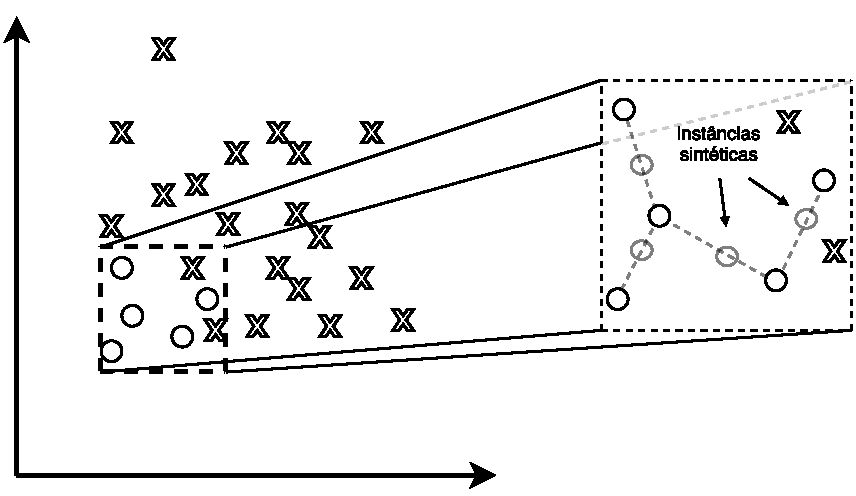
\includegraphics[width=0.7\linewidth]{figuras/smote.pdf}
  \end{center}
  \caption[Método SMOTE: interpolação entre dois exemplos vizinhos no espaço de características.]{Método SMOTE: interpolação entre dois exemplos vizinhos no espaço de características. \textit{Fonte: Elaborado pela autora.}}
  \label{fig:smote}
\end{figure}

Uma variação desse algoritmo, denominada Borderline-SMOTE1 \cite{Han2005}, considera que elementos fora da linha de borda de cada classe pouco contribuem para a classificação. Por isso, propôe a geração de elementos sintéticos utilizando apenas elementos de borda. Considera que se os vizinhos mais próximos são da classe majoritária, o exemplo é ruído, e se há mais vizinhos da classe majoritária do que da minoritária, considera esse elemento como sendo de borda. Como trabalho futuro, destacam a necessidade de considerar diferentes estratégias para definir em quais elementos realizar o over-sampling.


\subsection{Subamostragem}

Ao contrário da sobreamostragem, a subamostragem visa diminuir o número de elementos de um determinado conjunto. A ideia é eliminar elementos da classe majoritária que estão distantes da fronteira de decisão, isso porque eles são considerados menos relevantes para a aprendizagem.

Métodos para remoção de exemplos da classe majoritária normalmente apresentam resultados piores do que métodos de sobreamostragem, conforme relatado por \citeonline{Batista2004} e \citeonline{Japkowicz2002}. Um dos motivos pela preferência natural à sobreamostragem é o fato de que ao realizar subamostragem pode-se remover informações essenciais dos dados originais. Mas não há uma estratégia única que funcione melhor para todos os cenários.

%-------------------------------------------------------------------------------
\section{Classificador de padrões}
\label{sec:classificacao}

A tarefa de classificação de imagens consiste em tentar predizer a classe de uma determinada imagem. Na etapa de treinamento o método recebe como entrada um conjunto de imagens rotulado com suas respectivas classes; com o modelo treinado é possível realizar a classificação de exemplos de rótulo desconhecido; num experimento são preditas as classes de um conjunto de imagens de teste.

% \subsection{Naive Bayes}

% Os métodos probabilísticos bayesianos definem que a probabilidade de classificar um objeto como sendo de uma classe não depende apenas da relação entre eles, mas também  de observar a independência entre eles \cite{Faceli2011}. O teorema de Bayes é utilizado para calcular a probabilidade de um objeto $B$ pertencer a uma classe $A$:

% \begin{equation}
% P(A|B) = P(B|A)P(A)/P(B)
% \end{equation}

% \noindent onde $P(A|B)$ é a probabilidade de um exemplo $B$ pertencer à classe $A$; $P(A)$ a probabilidade ``a priori'' da classe e $P(B)$ que pode ser estimado pela frequência com que um novo exemplo ocorre, que pode ser ignorado por ser o mesmo para todas as classes \cite{Faceli2011}.

\subsection{\textit{K-Nearest Neighbors}}
\label{sec:knn}

O classificador \sigla{K-NN}{\textit{K-Nearest Neighbors}} considera a proximidade entre os dados para realizar predições. Baseia-se na premissa de que os objetos do mesmo conceito são semelhantes. O seu funcionamento está descrito no Algoritmo \ref{alg:knn}. Na fase de treinamento, apenas armazena os exemplos rotulados do conjunto de dados de treinamento. Quando um novo exemplo deve ser classificado, calcula a distância entre os vetores de características do novo exemplo e aqueles já rotulados. O novo exemplo é então classificado como sendo da classe do exemplo de treinamento com menor distância~\cite{Boiman2008}.

\begin{algorithm}[!htbp]
  \caption{K-NN: método de classificação supervisionada}
  \label{alg:knn}
  \SetAlgoLined
  \Entrada{Conjunto de exemplos $S_{treino}$ e $S_{teste}$}
  \Saida{Classes $C$ dos exemplos de teste preditas}
  $C \gets \emptyset $\;
  \ParaCada{teste $ \in S_{teste}$}{
    $N \gets k \text{ vizinhos mais próximos} (teste, S_{treino}) $\;
    $D \gets \emptyset $\;
    \ParaCada{vizinho $n \in N$}{
      $D \gets D \cup \text{distância} (n, teste) $\;
    }
    $C \gets C \cup menor(D)$\;
  }
\end{algorithm}

Com $K = 1$, a predição da classe corresponde ao exemplo mais próximo. Ao contrário de classificadores ``caixa preta'' (e.g. redes neurais), esse classificador permite o acompanhamento e análise do espaço de características representativo das imagens. Ao mesmo tempo, trata-se de um classificador que salienta a diferença entre as classes.

\meutodo{Adicionar uma seção apresentando o classificador SVM? Já que ele é
usado nos experimentos de quantização.}

%-------------------------------------------------------------------------------
\section{Redução de dimensionalidade}
\label{sec:reducaodimensionalidade}
% http://ieeexplore.ieee.org/stamp/stamp.jsp?tp=&arnumber=4368165

A visualização do espaço de características obtido após a geração artificial de imagens pode ajudar a verificar se as novas imagens melhoram a definição da classe minoritária em relação ao espaço original (inclusive antes de imagens serem removidas para provocar o desbalanceamento). Ou seja, se o método utilizado revelou características latentes. Dessa forma, ao projetar os novos vetores no espaço das imagens originais, é possível analisar qual método -- SMOTE ou geração de imagens no campo visual -- mais se assemelha à distribuição original dos dados.

Considerando que um vetor de características extraído com extratores comuns pode possuir entre 6 (e.g.\ Haralick) e 512 (e.g.\ BIC) características, a visualização de um exemplo requer que seja realizado o mapeamento desses valores em apenas duas dimensões. Para isso, uma redução de dimensionalidade mapeia os vetores de $N$ dimensões para um espaço 1D, 2D ou 3D. A partir desses novos vetores, pode então ser criada alguma representação visual que tente manter a relação de distância entre os novos e os originais~\cite{Paulovich2007}.

%%%%%%%%%%%%%%%%%%%%%%%%%%%%%%%%%%%%%%%%%%%%%%%%%%%%%%%%%%%%%%%%%%%%%%%%%%%%%%%%
\subsection{Análise de componentes principais}
\label{sec:pca}

% http://sebastianraschka.com/Articles/2014_pca_step_by_step.html
% http://arxiv.org/pdf/1404.1100v1.pdf

O \sigla{PCA}{\textit{Principal Component Analysis}} é uma técnica não supervisionada que pode ser utilizada para reduzir a dimensionalidade dos dados com a máxima variância possível. Cada imagem, originalmente representada por um vetor com $N$ características, pode então ser representada por apenas um ou mais valores. Essa redução permite a projeção dessas imagens no espaço de características. O objetivo é extrair as informações mais importantes dos dados e representá-las como um conjunto de variáveis ortogonais chamadas de componentes principais. Para isso encontra-se uma outra base: uma combinação linear da base original, que melhor representa os dados ao assumir que as direções das maiores variâncias são as mais importantes. Ou seja, a variância associada com cada direção quantifica o quão principal é aquela direção \cite{Abdi2010}. Pode-se, portanto, enumerar os passos necessários para o PCA sendo:

\begin{enumerate}
\item Centraliza todos os atributos na origem ao subtrair a média de cada dimensão;
\item Calcula a matriz de covariância $C_x$ dada por
\begin{equation}
    C_x = X X^T,
\end{equation}
\noindent onde $X$ é a matriz de dados original e $X^T$ sua transposta;

\item Encontra os autovalores e autovetores de $C_x$. Um autovetor $\vec{u}$ de uma matriz $A$ pode ser definido por $A\vec{u} = \lambda \vec{u}$, onde $\lambda$ é um autovalor escalar associado ao autovetor. Um vetor $\vec{u}$ é um autovetor da matriz $A$ se o tamanho do vetor -- e não sua direção -- é modificado quando multiplicado por $A$. Os autovalores podem ser representados na diagonal de uma matriz $\lambda$ (com outros valores como zero) e o conjunto dos autovetores de $A$ em uma matriz $U$. Assim,

\begin{equation}
    A = U \lambda U^T;
\end{equation}

\item Então, os autovetores são ordenados de forma decrescente de acordo com seus autovalores correspondentes e escolhe-se os $k$ principais autovetores (i.e.\ maiores autovalores) para formar uma matriz $P$ de dimensão $n \times k$, onde cada coluna representa um autovetor. O valor $k$ será a quantidade de dimensões do novo espaço de atributos;
 % O novo espaço de atributos pode ser encontrado multiplicando a transposta dessa matriz pela transposta dos atributos originais. - caso seja svd
\item O novo subespaço pode ser encontrado multiplicando essa matriz $P$ pela matriz original, de acordo com a equação $Y = PX$, onde $X$ representa o conjunto de dados original, $Y$ é uma nova representação desses dados e $P$ a matriz ortonormal que transforma $X$ em $Y$. As linhas de $P$ são os componentes principais de $X$.
\end{enumerate}

%%%%%%%%%%%%%%%%%%%%%%%%%%%%%%%%%%%%%%%%%%%%%%%%%%%%%%%%%%%%%%%%%%%%%%%%%%%%%%%%
\subsection{\textit{Locality preserving projections}}
\label{sec:lpp}

\sigla{LPP}{\textit{Locality preserving projections}} é um algoritmo linear de redução de dimensionalidade com propriedades de preservação da estrutura local dos dados. Não apresenta a dificuldade dos algoritmos tradicionais (como PCA) de manter o \textit{manifold} não linear dos dados originais \cite{Zhuo2014}. Embora o método mais utilizado para redução da dimensionalidade de forma não-supervisionada seja o PCA, métodos como esse produzem melhores projeções em termos de separação das classes. Em \citeonline{Zhuo2014} o LPP alcançou a melhor relação entre complexidade computacional e a redução da dimensionalidade, enquanto manteve a acurácia. Seu algoritmo segue três passos principais \cite{He2004}:

\begin{enumerate}
\item Constrói um grafo de adjacências. Os nós $i$ e $j$ possuem uma aresta entre si se fazem parte do conjunto de $k$-vizinhos mais próximos de cada nó (sendo $k$ um parâmetro do algoritmo);

\item Encontra os pesos $W_{ij} = 1$ se os vértices $i$ e $j$ estão próximos, ou seja, conectados por uma aresta, e $W_ij = 0$ caso contrário;

\item Computa os autovalores e autovetores
\begin{equation}
    X L X^T \vec{a} = \lambda X D X^T \vec{a},
\end{equation}
\noindent onde $D$ é a matriz diagonal na qual seus elementos são as somas das colunas de $W$ e $L$ é a matriz Laplaciana $L = D - W$. $X$ é a matriz original dos dados e $\vec{a}$ é o vetor solução (matriz de projeção), ordenado pelos autovalores $\lambda$.
\end{enumerate}

\meutodo{Adicionar as métricas estatísticas aqui? Ou deixar nos resultados? Precisa falar sobre ANOVA e HSD de Tukey?}

%--------------------------------------------------------------------------------
\section{Considerações finais}

Deu-se destaque à discussão das etapas de pré-processamento para a quantização de imagens, além das abordagens existentes para o rebalanceamento de classes. Esse capítulo apresentou métodos para exemplificação, além de trabalhos relacionados. A extração de características foi abordada, apresentando os principais descritores utilizados nesta pesquisa. A lacuna destacada é que existem características não passíveis de extração por descritores convencionais. Esses fundamentos permitem compreender o contexto no qual esta dissertação está inserida. Os próximos capítulos abrangem a metodologia proposta.

% Para isso, as redes de convolução são apresentadas, pois possuem capacidade de aprender as características relevantes das imagens de entrada. Justificando, assim, seu uso para análise das propriedades das bases de imagens. Podem também indicar possíveis operações para auxiliar na geração de imagens artificiais. Ainda, a memória associativa aprendida por máquinas de Boltzmann restritas pode ser indicadora de quais imagens geradas adicionam informações ao aprendizado.
%A geração dessas imagens visa rebalancear classes que diferem em número de imagens, e detalhes sobre esse problema também foram fundamentados nesse capítulo.
